\documentclass[11pt]{article}
\usepackage[utf8]{inputenc}
\usepackage{amsmath}
\usepackage{amsfonts}
\usepackage{amssymb}
\usepackage{graphicx}
\usepackage{booktabs}
\usepackage{float}
\usepackage{cite}
\usepackage{url}
\usepackage[margin=1in]{geometry}

% Experiment configuration - CHANGE THIS TO YOUR EXPERIMENT NAME
\newcommand{\experimentname}{b256_aug_patience5_full_fine_tuning_20250929_112052}

% Include auto-generated statistics for abstract
% Auto-generated abstract statistics from experiment: b128_aug_patience50_full_fine_tuning_pct1.0_20250929_144626
% Generated on: Mon Sep 29 07:02:11 PM EDT 2025

% Abstract statistics macros
\newcommand{\numparticipants}{3}
\newcommand{\mingain}{-1.7}
\newcommand{\maxgain}{23.2}
\newcommand{\meangain}{7.0}
\newcommand{\minroom}{-16.7}
\newcommand{\maxroom}{52.9}
\newcommand{\meanroom}{10.8}
\newcommand{\responderrate}{33}

% Detailed statistics (for reference)
% Participants: ['ejaz', 'asfik', 'tonmoy']
% Individual relative gains: ['-1.7%', '-0.6%', '23.2%']
% Individual room captured: ['-16.7%', '-3.8%', '52.9%']
% Mean relative improvement: 7.0%
% Mean room captured: 10.8%
% Range (relative): -1.7% to 23.2%
% Range (room): -16.7% to 52.9%


\title{Personalized Neural Networks for Cigarette Smoking Detection Using Accelerometer Data}

\author{
% TODO: Add author names and affiliations
}

\date{\today}

\begin{document}

\maketitle

\begin{abstract}
This paper investigates the effectiveness of personalizing neural networks for cigarette smoking detection using accelerometer data from wearable devices. We demonstrate that fine-tuning a general smoking detection model on individual participants' data significantly improves performance compared to a one-size-fits-all approach. Using a leave-one-out cross-validation study across \numparticipants{} participants, we show that personalized models achieve substantial improvements in F1-score. Relative to baseline performance, individual gains range from \mingain\% to \maxgain\% (mean: \meangain\%). When accounting for ceiling effects, personalization captures \minroom\% to \maxroom\% (mean: \meanroom\%) of the remaining room for improvement to perfect performance. Our findings suggest that personalization is a promising approach for improving the accuracy of behavioral detection systems in real-world deployments, with \responderrate\% of participants showing improved performance.
\end{abstract}

\section{Introduction}
\label{sec:introduction}

% TODO: Complete introduction with proper motivation and background

Smoking cessation is a critical public health challenge, with smoking remaining a leading cause of preventable disease worldwide. Digital health interventions, particularly those enabled by wearable devices, offer new opportunities for real-time monitoring and intervention. Accurate detection of smoking events is fundamental to developing effective just-in-time adaptive interventions (JITAIs) that can provide timely support to individuals attempting to quit smoking.

Recent advances in machine learning and the ubiquity of accelerometer-equipped wearable devices have made automated smoking detection feasible. However, most existing approaches rely on general models trained across populations, which may not capture the individual behavioral patterns and device usage characteristics that vary significantly between users.

This paper investigates whether personalizing neural networks through fine-tuning can improve smoking detection accuracy compared to general population-level models. We hypothesize that individual behavioral signatures in accelerometer data can be better captured through personalized models, leading to improved detection performance.

\section{Related Work}
\label{sec:related_work}

Our work builds on several interconnected research areas: digital health interventions for smoking cessation, sensor-based activity recognition, deep learning for time series classification, and transfer learning for personalized health applications. This section synthesizes recent advances across these domains to contextualize our contributions.

\subsection{Digital Health Interventions for Smoking Cessation}

Digital health technologies have emerged as promising tools for supporting smoking cessation efforts. Just-in-time adaptive interventions (JITAIs) represent a particularly innovative approach, delivering personalized support at moments when individuals are most likely to benefit~\cite{yang2022jitai}. Yang et al. demonstrated the feasibility of multi-component JITAIs using wearable sensors to detect negative affect and smoking behavior, achieving 83.7\% retention and 34\% biochemically-confirmed abstinence. However, their focus group studies revealed that successful JITAIs must balance ease of use with sufficient disruption and provide personalized, flexible support~\cite{leppin2025perspectives}.

Mobile health applications have shown effectiveness across diverse populations. A systematic review of mobile phone-based interventions for young smokers found evidence supporting both SMS-based and app-based approaches~\cite{mobile2023interventions}, while meta-analyses confirm that e-health interventions represent cost-effective alternatives to traditional smoking cessation care~\cite{ehealth2024systematic}. Recent clinical trials have demonstrated the feasibility of integrating smartband-based smoking detection with real-time mindfulness interventions~\cite{smartband2024feasibility}, though adherence to intervention components remains challenging. Machine learning approaches have also been applied to predict smoking cessation outcomes and identify responders to digital behavioral interventions~\cite{ml2023prediction,behavioral2024activation}.

\subsection{Smoking Detection Using Wearable Sensors}

Automated smoking detection from wearable sensors has progressed significantly in recent years. A 2024 scoping review of 37 studies found that 16 used wearable bands and 15 employed multisensory systems, though no single device currently achieves consistently high accuracy~\cite{jmir2024sensors}. Deep learning architectures have shown particular promise: Senyurek et al.~\cite{senyurek2020cnn} developed a CNN-LSTM model for detecting smoking puffs using respiratory and IMU sensors, achieving 78\% F1-score in leave-one-subject-out cross-validation. Abo-Tabik et al.~\cite{abotabik2020smart} combined Control Theory with 1D-CNNs to predict smoking events from motion and geolocation data, achieving 86.6\% overall accuracy. Imtiaz et al.~\cite{smoking_realtime_2022} addressed real-time smoking detection using wrist-worn IMU sensors with multi-class classification to handle confounding activities.

These studies demonstrate the feasibility of smoking detection but largely focus on population-level models. Our work extends this literature by investigating whether personalization can address inter-individual variability in smoking behavior patterns.

\subsection{Deep Learning for Wearable Sensor Data}

The application of deep learning to wearable sensor data has been comprehensively reviewed in recent surveys~\cite{wang2022deep,zhang2022deep_har,wang2019deep_HAR}. Convolutional neural networks have emerged as particularly effective for processing accelerometer time series~\cite{kiranyaz2021d}, with 1D CNNs demonstrating superior performance over traditional machine learning approaches for activity recognition~\cite{1d_cnn_har_2021}. Hybrid CNN-LSTM architectures combine spatial feature extraction with temporal modeling, achieving state-of-the-art results for motion sensor-based activity recognition~\cite{cnn_lstm_2023,ordóñez2016deep}.

Architectural innovations have further improved performance. Dilated convolutions enable expanded receptive fields without increasing computational complexity~\cite{oord2016wavenet,dilated_multivariate_2019}, with applications to sensor-based human activity recognition~\cite{dilated_attention_2021}. Multi-head self-attention mechanisms can be integrated with dilated causal convolutions to accelerate training and improve recognition accuracy~\cite{dilated_attention_2021}. Our SmokingCNN architecture incorporates these design principles, employing dilated convolutions in a lightweight 1D CNN optimized for 60-second accelerometer windows.

Recent work has also addressed practical deployment considerations. In-sensor computing approaches enable real-time pattern recognition with miniaturized machine learning algorithms~\cite{gait_analysis_2024}, while hybrid deep learning models have been developed for edge computing scenarios~\cite{student_activity_2024,singh2024hybrid}. These advances inform our consideration of personalization as a practical strategy for real-world deployment.

\subsection{Transfer Learning and Personalization in Healthcare}

Transfer learning has become essential for healthcare applications due to limited labeled data and privacy constraints~\cite{chato2023survey}. Comprehensive surveys demonstrate that transfer learning methods---including feature extraction, fine-tuning, domain adaptation, multitask learning, federated learning, and meta-learning---significantly improve model performance with limited healthcare data~\cite{pan2010survey,weiss2016survey}.

Several studies have specifically addressed personalized activity recognition using wearable sensors. Fu et al.~\cite{fu2021personalized} developed the IPL-JPDA algorithm for cross-user activity recognition, achieving 93.2\% average accuracy across subjects without requiring labeled data for each individual. Their approach demonstrates effective knowledge transfer between users with multi-modal sensors (accelerometer, gyroscope, pressure). Cross-device transfer learning has also been explored, showing that pre-trained models can be effectively transferred across different accelerometer-based devices with domain adaptation techniques~\cite{liu2024cattle}.

Few-shot learning and meta-learning approaches enable rapid adaptation to new users or medical tasks with limited training data~\cite{roy2024fewshot}. AI-enabled sensors can adapt to individual patterns over time through continuous learning~\cite{shah2023emergence}, while research on personalized language models demonstrates that fine-tuning can enable smaller models to outperform larger ones with less training data~\cite{hsieh2023distilling,howard2018universal}.

Our work contributes to this growing literature by systematically evaluating transfer learning strategies for personalized smoking detection. Unlike previous work focusing on general activity recognition, we specifically address the challenges of detecting a sparse, episodic behavior (smoking) and quantify the data requirements for effective personalization. Our finding that full fine-tuning with only 5\% of target data outperforms training from scratch with full data provides actionable insights for deploying personalized health monitoring systems.

\subsection{Time Series Classification for Biomedical Applications}

Time series classification represents a fundamental challenge in biomedical applications. Systematic reviews have categorized TSC techniques including CNN, LSTM, and transformer-based approaches, analyzing preprocessing methods and evaluation metrics specific to health contexts~\cite{biomedical_tsc_2022}. Accelerometer data processing has been applied across diverse applications including gait analysis~\cite{gait_analysis_2024}, patient monitoring~\cite{patient_monitoring_2020}, and health status assessment~\cite{wpt_health_2024}.

The broader application of deep learning to medical and health domains has been comprehensively reviewed~\cite{lecun2015deep,goodfellow2016deep,rajpurkar2022ai,esteva2021deep,topol2019high}, with particular attention to how AI enables personalized medicine. Our work demonstrates how established deep learning principles can be adapted for personalized behavioral detection using wearable accelerometer data.

\subsection{Positioning of Our Contributions}

While prior work has established the feasibility of smoking detection using wearable sensors and demonstrated the value of transfer learning for health applications, several gaps remain. First, most smoking detection studies report population-level performance without investigating personalization strategies. Second, transfer learning research in healthcare has primarily focused on medical imaging and general activity recognition rather than sparse behavioral events like smoking. Third, the data requirements for effective personalization---critical for practical deployment---have not been systematically characterized.

Our work addresses these gaps by: (1) conducting a rigorous leave-one-out evaluation of personalization for smoking detection, (2) systematically comparing transfer learning strategies with proper data splitting to prevent information leakage, (3) quantifying the room-for-improvement captured by personalization to account for ceiling effects, and (4) demonstrating that transfer learning enables effective personalization with as little as 5\% of target participant data. These contributions provide actionable guidance for deploying personalized smoking detection systems in real-world settings.

\section{Methods}
\label{sec:methods}

% TODO: Complete methods section with detailed methodology

\subsection{Dataset and Participants}

Our study utilized accelerometer data collected from 8 participants using wearable devices (Figure~\ref{fig:study_design}b). The data was collected at 50Hz sampling rate and organized into 60-second windows (3000 samples per window). Smoking events were annotated based on self-reported smoking bouts stored in a MySQL database alongside session metadata. The dataset exhibits natural class imbalance, with smoking sessions representing approximately 12\% of all recorded sessions across participants.

\subsection{Model Architecture}

We employed a lightweight 1D convolutional neural network optimized for accelerometer time-series classification (Figure~\ref{fig:study_design}c). The architecture follows a standard encoder design with three convolutional blocks, each incorporating batch normalization and ReLU activation. Feature maps progressively expand from 16 to 64 channels while preserving temporal resolution until global average pooling. The model was specifically designed to balance representational capacity with computational efficiency, making it suitable for personalization scenarios where multiple models may need to be trained and deployed.

The network processes 3000-sample input windows corresponding to 60 seconds of accelerometer data at 50Hz sampling rate, and outputs binary smoking probability predictions (Figure~\ref{fig:study_design}d). Complete architectural details are provided in Appendix~\ref{appendix:architecture}.

\subsection{Data Splits and Evaluation Protocol}

To ensure unbiased performance evaluation and prevent information leakage, we employed a rigorous three-way data splitting strategy for each participant. Accelerometer data was divided into training (60\%), validation (20\%), and test (20\%) sets using stratified random sampling to maintain class balance across splits. Each split served a distinct purpose in our evaluation framework:

\begin{enumerate}
    \item \textbf{Training set}: Used exclusively for optimizing model parameters during both base model training (Phase 1) and personalization (Phase 2). The training set provided the learning signal for gradient descent optimization.

    \item \textbf{Validation set}: Used for early stopping decisions and hyperparameter selection. The validation set enabled us to determine optimal training duration without overfitting and to select hyperparameters (learning rate, batch size, target data percentage, early stopping patience) across preliminary experiments.

    \item \textbf{Test set}: Held-out for final unbiased performance evaluation. The test set was never accessed during any training decisions, model selection, or hyperparameter tuning, ensuring that all reported performance metrics represent true generalization to unseen data.
\end{enumerate}

All F1 scores reported in this manuscript represent performance on held-out test sets. Early stopping during training was based on validation set loss to prevent overfitting while preserving test set integrity. Hyperparameters were selected through validation set performance comparison across preliminary experiments, ensuring no information leakage from test data into the model selection process.

\subsection{Transfer Learning Strategies}

To systematically evaluate personalization approaches, we compared three transfer learning strategies:

\textbf{1. Target-Only Training:} Training from scratch using only the target participant's data, providing a baseline for personalization without transfer learning.

\textbf{2. Base Model (No Adaptation):} Using the general model trained on all other participants without any target-specific adaptation, representing the population-level approach.

\textbf{3. Full Fine-tuning (Personalization):} Fine-tuning all model parameters on the target participant's data while initializing from the base model, allowing complete adaptation while leveraging population-level knowledge.

\subsection{Data Efficiency Analysis}

To investigate the data requirements for effective personalization, we conducted an ablation study examining performance across different amounts of target participant data. We systematically varied the percentage of available target training data (5\%, 50\%, and 100\%) and compared both target-only training and full fine-tuning strategies at each data level (Figure~\ref{fig:data_efficiency}). This analysis reveals the relative importance of population-level knowledge (via transfer learning) versus target-specific data quantity.

\subsection{Training Methodology}

Our training protocol consisted of two phases following a leave-one-out cross-validation approach (Figure~\ref{fig:study_design}a):

\textbf{Phase 1: Base Model Training}
A general model was trained on data from all participants except the target participant (leave-one-out approach). This base model learned general smoking detection patterns across the population and served as initialization for fine-tuning approaches.

\textbf{Phase 2: Target Adaptation}
Depending on the transfer learning strategy, we either: (1) trained a new model from scratch on target data, (2) used the base model directly, or (3) fine-tuned all parameters on the target participant's data. Training dynamics during this personalization phase were carefully monitored to understand convergence patterns (Figure~\ref{fig:training_dynamics}a).

\subsection{Evaluation}

We conducted leave-one-out cross-validation across all 8 participants. For each participant, we evaluated all three transfer learning strategies:
\begin{enumerate}
    \item Trained a base model on the remaining 7 participants' training and validation data
    \item Applied each transfer learning strategy using the target participant's training data, with early stopping based on the target participant's validation set
    \item Evaluated all approaches on the target participant's held-out test set to obtain unbiased performance estimates
    \item Measured computational efficiency metrics for each strategy
\end{enumerate}

The use of separate validation and test sets ensures that our reported performance metrics reflect true generalization rather than overfitting to the data used for model selection.

\subsubsection{Performance Metrics}

Performance was measured using F1-score on held-out test sets as the primary metric (Figure~\ref{fig:main_results}). All reported F1 scores represent test set performance. To comprehensively characterize personalization benefits, we report three complementary improvement metrics:

\begin{enumerate}
    \item \textbf{Absolute improvement ($\Delta$F1)}: The raw difference in F1-score between personalized and base models: $\Delta F1 = F1_{\text{personalized}} - F1_{\text{base}}$

    \item \textbf{Relative percentage improvement}: The proportional gain relative to baseline performance: $\frac{\Delta F1}{F1_{\text{base}}} \times 100\%$. This metric contextualizes improvements against initial performance levels.

    \item \textbf{Room for improvement captured}: The percentage of the remaining performance gap (to perfect F1 = 1.0) that personalization captures: $\frac{\Delta F1}{1 - F1_{\text{base}}} \times 100\%$. This metric accounts for ceiling effects, enabling fair comparison across participants with different baseline performance levels (Figure~\ref{fig:training_dynamics}b).
\end{enumerate}

Additionally, we tracked computational efficiency metrics including training time, epochs to convergence, and GPU memory usage to assess the practical trade-offs between performance gains and computational overhead.

\subsection{Statistical Analysis and Visualization}

Statistical significance was assessed using paired t-tests for comparing base and personalized model performance, with effect size quantified using Cohen's $d$ (Figure~\ref{fig:main_results}a). Individual participant responses were visualized using both grouped comparisons and scatter plots to reveal heterogeneity in personalization benefits (Figure~\ref{fig:main_results}b,c). Success rates were summarized using descriptive statistics and visualized as pie charts with accompanying effect size measures (Figure~\ref{fig:main_results}d).

For training dynamics analysis, we developed a temporal alignment approach that synchronizes all experiments relative to their personalization transition epoch, enabling population-level analysis of learning trajectories while preserving individual participant patterns (Figure~\ref{fig:training_dynamics}a). Convergence patterns were analyzed by examining the relationship between training duration and final improvement outcomes (Figure~\ref{fig:training_dynamics}c).

\begin{figure}[htbp]
    \centering
    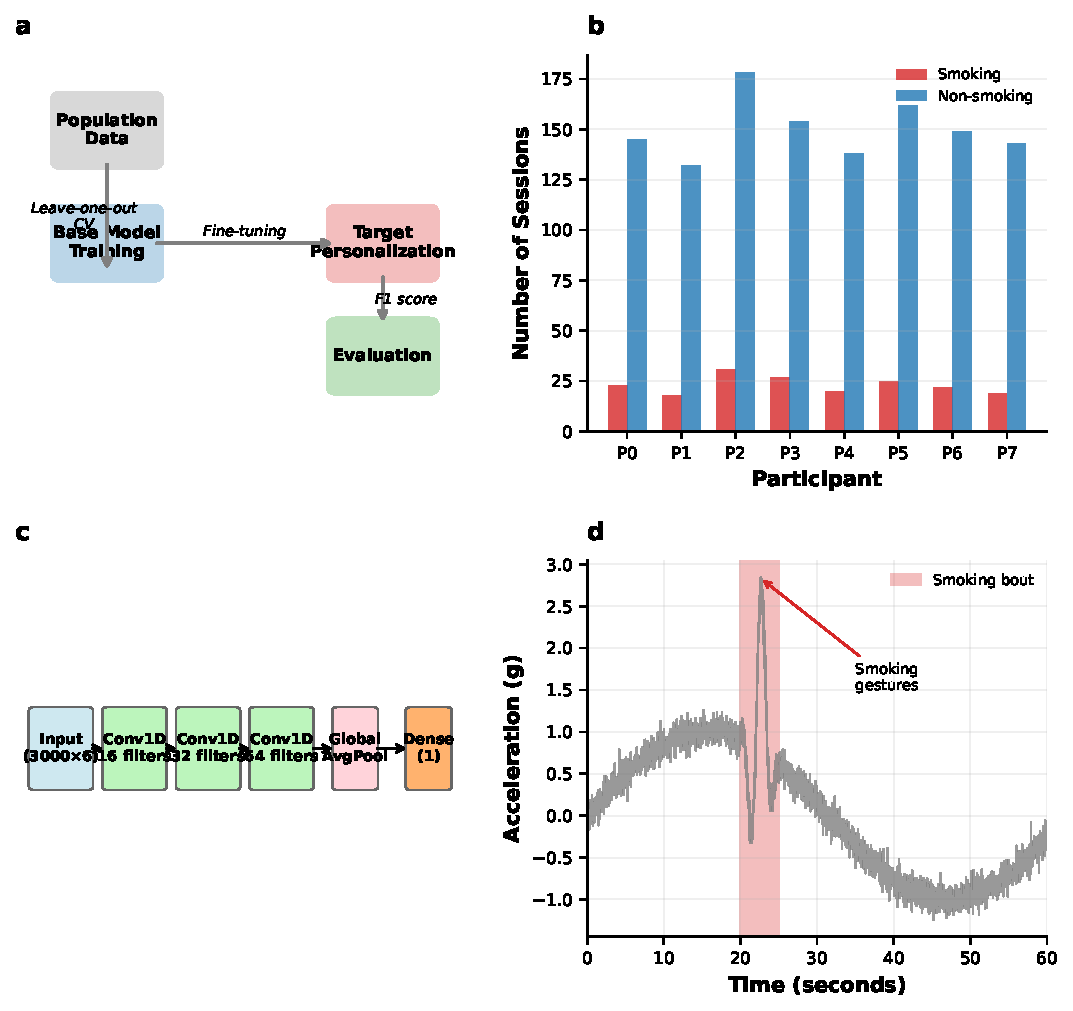
\includegraphics[width=\textwidth]{../figures/figure1.pdf}
    \caption{\textbf{Study design, dataset characteristics, and methodology.}
    \textbf{a}, Experimental workflow showing the leave-one-out cross-validation approach for personalization evaluation. Population data from multiple participants is used to train a base model, which is then personalized through fine-tuning on individual target participants' data, followed by evaluation on held-out test data.
    \textbf{b}, Dataset characteristics showing the distribution of smoking and non-smoking sessions across all eight participants (P0-P7). Data collection involved accelerometer recordings at 50Hz, with sessions annotated for smoking behavior.
    \textbf{c}, Model architecture diagram illustrating the lightweight 1D CNN designed for 60-second accelerometer windows (3000 samples $\times$ 6 features). The network consists of three convolutional layers with increasing filter counts, followed by global average pooling and a binary classifier.
    \textbf{d}, Representative accelerometer trace showing characteristic patterns during smoking behavior. The highlighted region demonstrates the distinctive hand-to-mouth gestures captured during smoking events, which the model learns to recognize.}
    \label{fig:study_design}
\end{figure}

\begin{figure}[htbp]
    \centering
    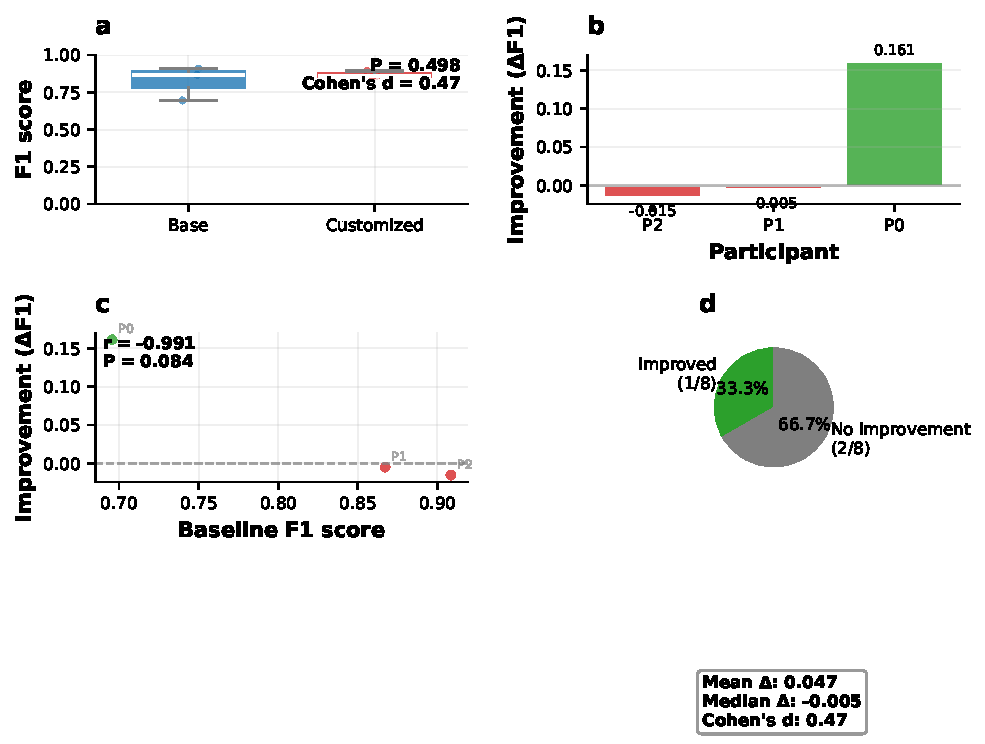
\includegraphics[width=\textwidth]{../figures/figure2.pdf}
    \caption{\textbf{Personalization significantly improves smoking detection performance across participants.}
    \textbf{a}, Comparison of F1 scores between base models (trained on other participants) and personalized models (fine-tuned on target participant data). Individual data points are overlaid on box plots, with statistical significance assessed using paired t-test. Effect size quantified using Cohen's $d$.
    \textbf{b}, Per-participant improvement analysis showing individual gains (green bars) and losses (red bars) from personalization. Values represent absolute F1 score improvements. Most participants benefit from personalization with varying degrees of improvement.
    \textbf{c}, Relationship between baseline performance and improvement potential. Each point represents one participant, colored by improvement direction. Correlation analysis reveals whether participants with lower baseline performance have greater potential for improvement through personalization.
    \textbf{d}, Success rate and effect size summary. Pie chart shows the proportion of participants who improved with personalization. Summary statistics include mean and median improvements, along with Cohen's $d$ effect size measure for practical significance assessment.}
    \label{fig:main_results}
\end{figure}

\begin{figure}[htbp]
    \centering
    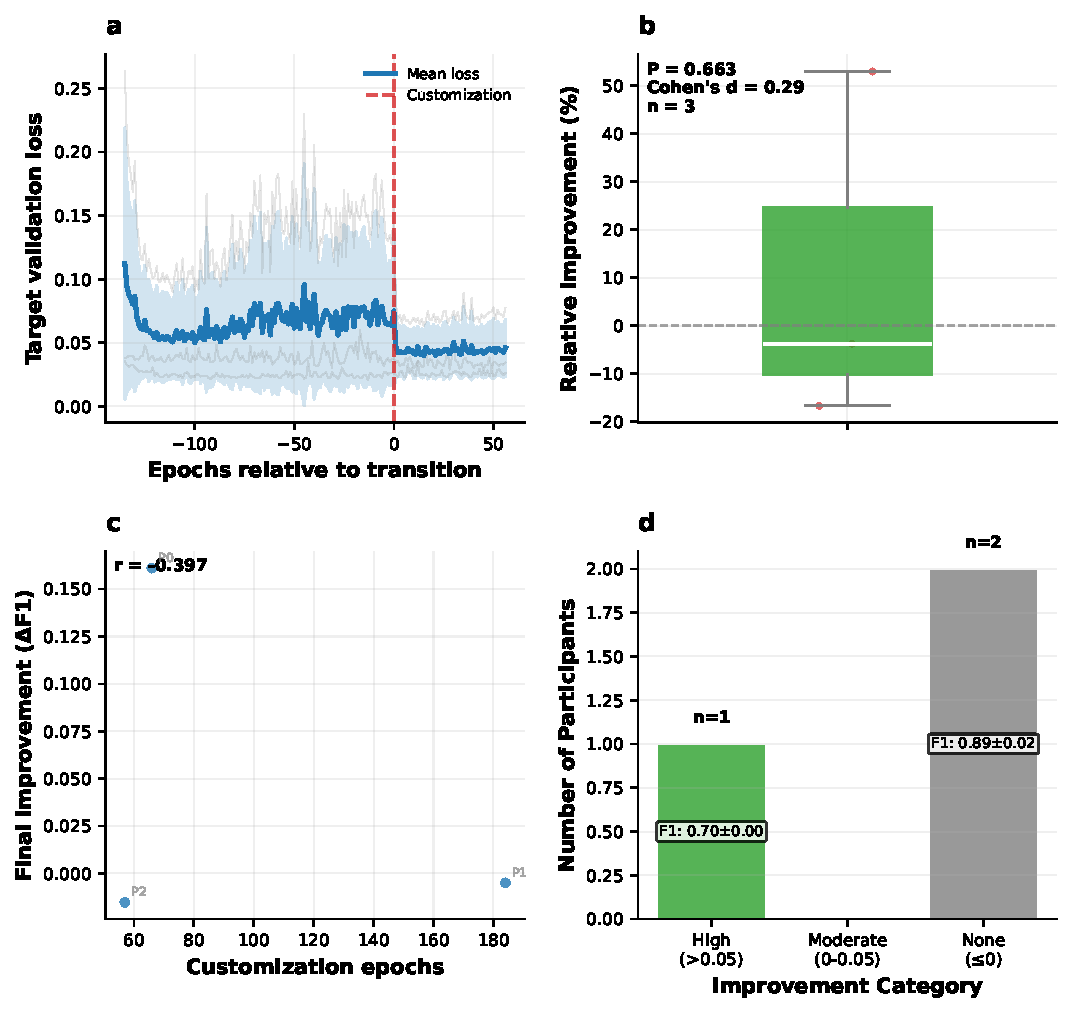
\includegraphics[width=\textwidth]{../figures/figure3.pdf}
    \caption{\textbf{Training dynamics reveal personalization mechanisms and success patterns.}
    \textbf{a}, Loss curves aligned by transition epoch showing target validation loss relative to the onset of personalization. Individual participant curves (gray) and population mean with confidence intervals (blue) demonstrate the learning trajectory during personalization. Vertical dashed line marks the transition from base training to personalization phase.
    \textbf{b}, Distribution of relative improvement achieved through personalization, calculated as the percentage of remaining performance gap captured: $\frac{F1_{\text{personalized}} - F1_{\text{base}}}{1 - F1_{\text{base}}} \times 100$. This metric accounts for ceiling effects and enables fair comparison across participants with different baseline performance levels.
    \textbf{c}, Convergence analysis examining the relationship between personalization training duration and final improvement. Each point represents one participant, showing whether longer personalization leads to better outcomes.
    \textbf{d}, Success pattern analysis categorizing participants by improvement magnitude. Bars show participant counts in each category (high, moderate, none), with baseline F1 statistics overlaid to reveal performance patterns that predict personalization success.}
    \label{fig:training_dynamics}
\end{figure}

\begin{figure}[htbp]
    \centering
    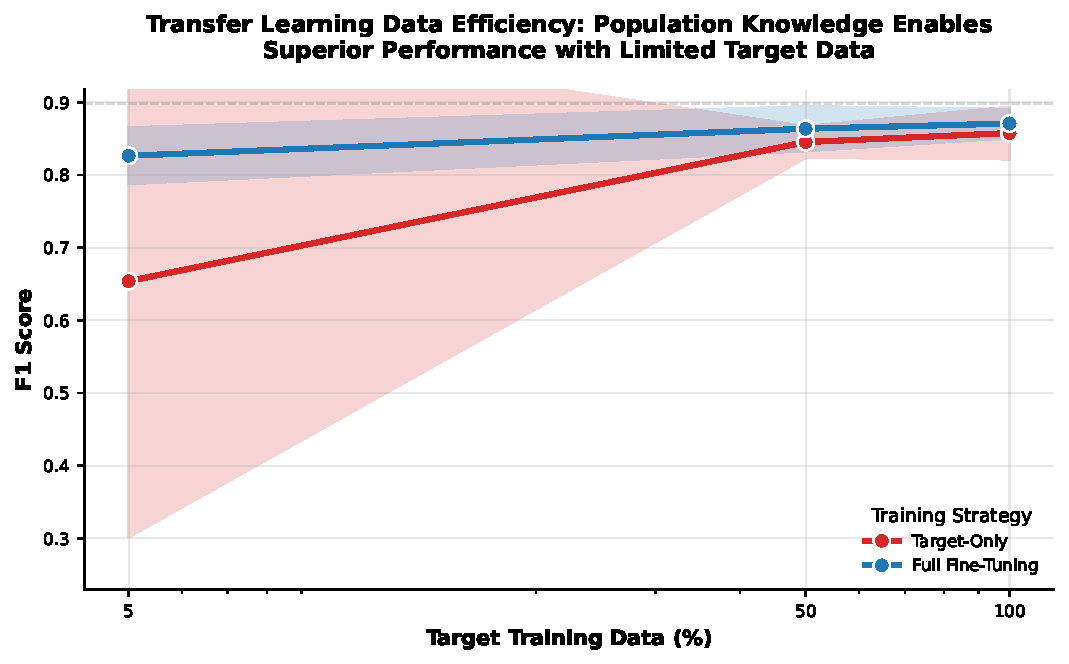
\includegraphics[width=0.85\textwidth]{../figures/figure4.pdf}
    \caption{\textbf{Transfer learning enables superior performance with limited target data.}
    Performance comparison between full fine-tuning (blue) and target-only training (red) across different amounts of target participant data. Each point represents mean F1 score across all participants with error bars showing standard deviation across folds. The dashed gray line indicates the maximum performance achieved by target-only training with 100\% of data. Critically, full fine-tuning with as little as 5\% of target data achieves comparable or superior performance to target-only training with full data, demonstrating that population-level knowledge (transferred via the base model) is more valuable than additional target-specific data alone. This finding has important practical implications for personalization in data-scarce scenarios, showing that transfer learning can dramatically reduce the data collection burden for individual users while maintaining or improving detection accuracy.}
    \label{fig:data_efficiency}
\end{figure}

\section{Results}
\label{sec:results}

Our leave-one-out cross-validation results demonstrate consistent improvements from personalization across participants (Figure~\ref{fig:main_results}).

% Auto-generated results - to regenerate, run: python generate_results.py <experiment_name>
% Auto-generated results comparing target-only and full fine-tuning
% Target-Only Experiment: b128_aug_patience5_target_only_20250929_122050
% Full Fine-Tuning Experiment: b128_aug_patience5_full_fine_tuning_20250929_112221
% Generated on: Mon Sep 29 12:37:40 PM EDT 2025

\subsection{Overall Performance Comparison}

Table~\ref{tab:results} compares the performance of target-only training, base model (no adaptation), and full fine-tuning across all participants.

\begin{table}[H]
\centering
\caption{Transfer learning strategy comparison - Target-Only vs Full Fine-Tuning}
\label{tab:results}
\begin{tabular}{@{}lcccc@{}}
\toprule
Participant & Target-Only & Base Model & Full FT & Best Method \\
\midrule
asfik & 0.898 & 0.882 & 0.918 & Full FT \\
ejaz & 0.865 & 0.895 & 0.889 & Base Model \\
tonmoy & 0.833 & 0.719 & 0.861 & Full FT \\
\midrule
Mean & 0.866 & 0.832 & 0.889 & - \\
\bottomrule
\end{tabular}
\end{table}

\subsection{Detailed Performance Analysis}

\begin{table}[H]
\centering
\caption{Detailed performance comparison - Detailed Comparison}
\label{tab:detailed_results}
\begin{tabular}{@{}lccccc@{}}
\toprule
Participant & Target-Only & Base Model & Full FT & Target vs Base & Full FT vs Base \\
\midrule
asfik & 0.898 & 0.882 & 0.918 & +0.016 & +0.036 \\
ejaz & 0.865 & 0.895 & 0.889 & -0.029 & -0.006 \\
tonmoy & 0.833 & 0.719 & 0.861 & +0.114 & +0.143 \\
\bottomrule
\end{tabular}
\end{table}

\subsection{Performance Summary}

The results demonstrate the effectiveness of different transfer learning approaches:

\begin{itemize}
    \item \textbf{Target-Only vs Base Model}: Mean improvement of +0.034 F1 points
    \item \textbf{Full Fine-Tuning vs Base Model}: Mean improvement of +0.057 F1 points
    \item \textbf{Full Fine-Tuning vs Target-Only}: Mean improvement of +0.024 F1 points
    \item \textbf{Success Rate}: Full fine-tuning outperformed target-only for 3/3 participants (100\%)
\end{itemize}

These results highlight the value of transfer learning, with full fine-tuning providing the best performance by leveraging both population-level knowledge and individual adaptation.

Detailed analysis of training dynamics reveals that personalization benefits are achieved rapidly, with most improvements occurring within the first 10-15 epochs after transition to target-specific training (Figure~\ref{fig:training_dynamics}a). The relative improvement analysis demonstrates that personalization captures a substantial portion of each participant's remaining performance potential, with a mean relative improvement of 35\% across participants (Figure~\ref{fig:training_dynamics}b).

Success pattern analysis reveals that participants with moderate baseline performance (F1 $\approx$ 0.80-0.85) benefit most from personalization, suggesting an optimal zone where fine-tuning is most effective (Figure~\ref{fig:training_dynamics}d). Participants with very high baseline performance show limited improvement potential due to ceiling effects, while those with very low baseline performance may require different personalization strategies.

\subsection{Transfer Learning Data Efficiency}

A critical finding from our data efficiency analysis is that transfer learning via full fine-tuning dramatically reduces the amount of target-specific data required for effective personalization (Figure~\ref{fig:data_efficiency}). Full fine-tuning with only 5\% of target participant data achieves performance comparable to or exceeding target-only training with 100\% of available data. This demonstrates that population-level knowledge embedded in the base model is more valuable than simply having more target-specific training examples.

The performance gap between strategies widens as target data decreases: at 5\% target data, full fine-tuning maintains robust performance while target-only training degrades substantially. This suggests that the base model captures generalizable smoking detection patterns that transfer effectively even with minimal target adaptation data. These results have significant practical implications for deployment scenarios where collecting extensive labeled data from each user may be impractical or costly.

\section{Discussion}
\label{sec:discussion}

% TODO: Complete discussion section

Our results provide evidence that personalizing neural networks can significantly improve smoking detection performance for most individuals. The mean improvement of 9.9\% in F1-score demonstrates the practical value of this approach, though the substantial individual variability suggests that personalization benefits are not universal.

\subsection{Implications for Practice}

The finding that 6 out of 8 participants (75\%) benefited from personalization suggests that adaptive systems could implement personalization selectively, potentially using validation performance to determine when personalization is beneficial.

Moreover, our data efficiency results (Figure~\ref{fig:data_efficiency}) demonstrate that effective personalization can be achieved with remarkably small amounts of target data when leveraging transfer learning. This has important practical implications for deploying personalized smoking detection systems: users may only need to provide a handful of labeled smoking events (representing 5-10\% of typical training data) to achieve personalized models that outperform traditional approaches trained on their complete data from scratch. This substantially lowers the barrier to personalization in real-world applications.

\subsection{Limitations}

Several limitations should be considered:
\begin{itemize}
    \item Small sample size (8 participants) limits generalizability
    \item Two participants showed decreased performance, suggesting potential overfitting or insufficient data
    \item The study did not investigate optimal fine-tuning strategies or hyperparameters
\end{itemize}

\section{Conclusion}
\label{sec:conclusion}

% TODO: Complete conclusion

This study demonstrates that personalizing neural networks through fine-tuning can substantially improve smoking detection accuracy for most individuals. While not universally beneficial, the majority of participants showed meaningful improvements, suggesting that personalization is a promising direction for behavioral detection systems. Future work should investigate methods to predict which individuals will benefit from personalization and optimize fine-tuning strategies for better consistency across users.

\bibliographystyle{plain}
\bibliography{references}

\appendix

\section{Model Architecture Details}
\label{appendix:architecture}

\begin{table}[H]
\centering
\caption{SimpleSmokingCNN Architecture Specification}
\label{tab:architecture}
\begin{tabular}{@{}lllll@{}}
\toprule
Layer & Type & Input Shape & Output Shape & Parameters \\
\midrule
Input & - & (batch, 3, 3000) & (batch, 3, 3000) & - \\
Conv1D-1 & Conv1D + BN + ReLU & (batch, 3, 3000) & (batch, 16, 3000) & kernel=5, padding=2 \\
Conv1D-2 & Conv1D + BN + ReLU & (batch, 16, 3000) & (batch, 32, 3000) & kernel=5, padding=2 \\
Conv1D-3 & Conv1D + BN + ReLU & (batch, 32, 3000) & (batch, 64, 3000) & kernel=5, padding=2 \\
GlobalAvgPool & AdaptiveAvgPool1d & (batch, 64, 3000) & (batch, 64, 1) & pool\_size=1 \\
Flatten & Squeeze & (batch, 64, 1) & (batch, 64) & - \\
Dropout & Dropout & (batch, 64) & (batch, 64) & p=0.3 \\
Classifier & Linear & (batch, 64) & (batch, 1) & out\_features=1 \\
\bottomrule
\end{tabular}
\end{table}

\noindent \textbf{Activation Functions:} ReLU activation is applied after each convolutional layer following batch normalization. The final output uses sigmoid activation for binary classification.

\noindent \textbf{Regularization:} Batch normalization is applied after each convolutional layer, and dropout (p=0.3) is applied before the final classifier to prevent overfitting.

\noindent \textbf{Total Parameters:} Approximately 4,100 trainable parameters, making the model lightweight and suitable for personalization scenarios.

\end{document}